\section{Central Neutron Detector (CND)}

\subsection{Geometry}

The CND geometry is implemented through the native gemc geometry API.
The paddles are Geant4 generic trapezoids, see \F{cndGeometry}. The scintillator junctions are G4Polycons.
The paddles are assigned the scintillator material and associated with the cnd hit process routine.

\begin{figure}
	\centering
	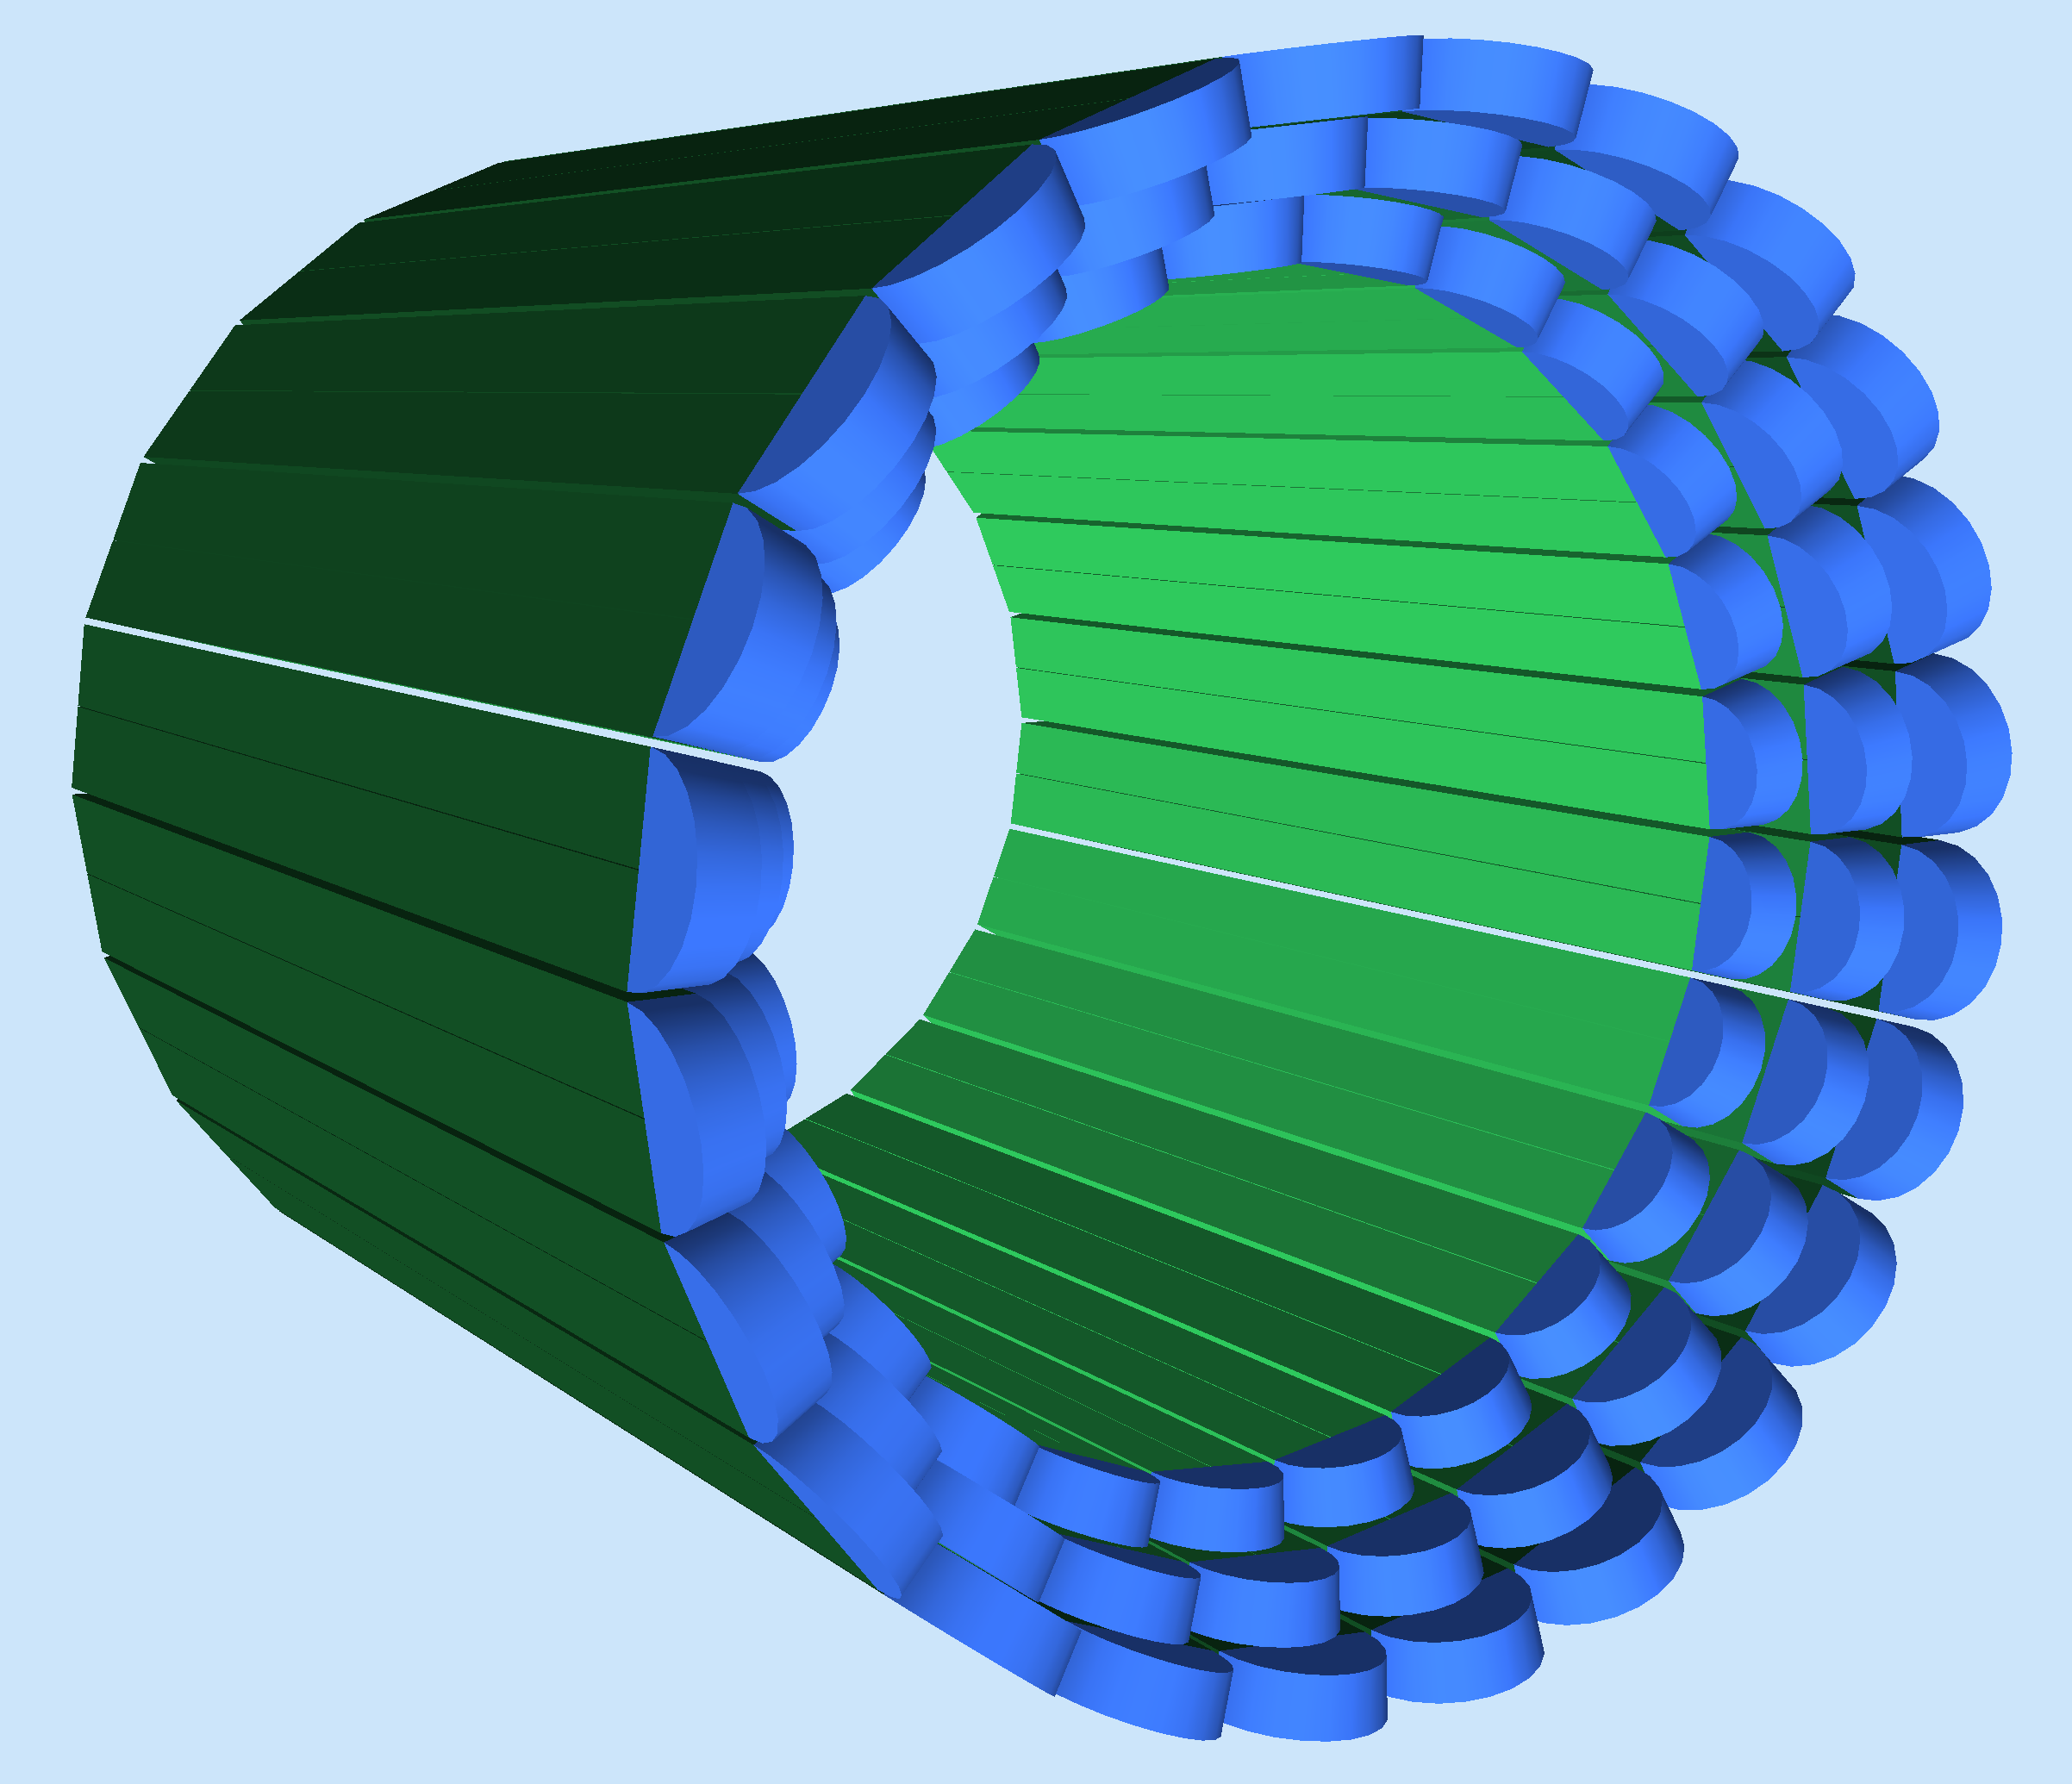
\includegraphics[width=0.95\columnwidth,keepaspectratio]{img/cndGeometry.png}
	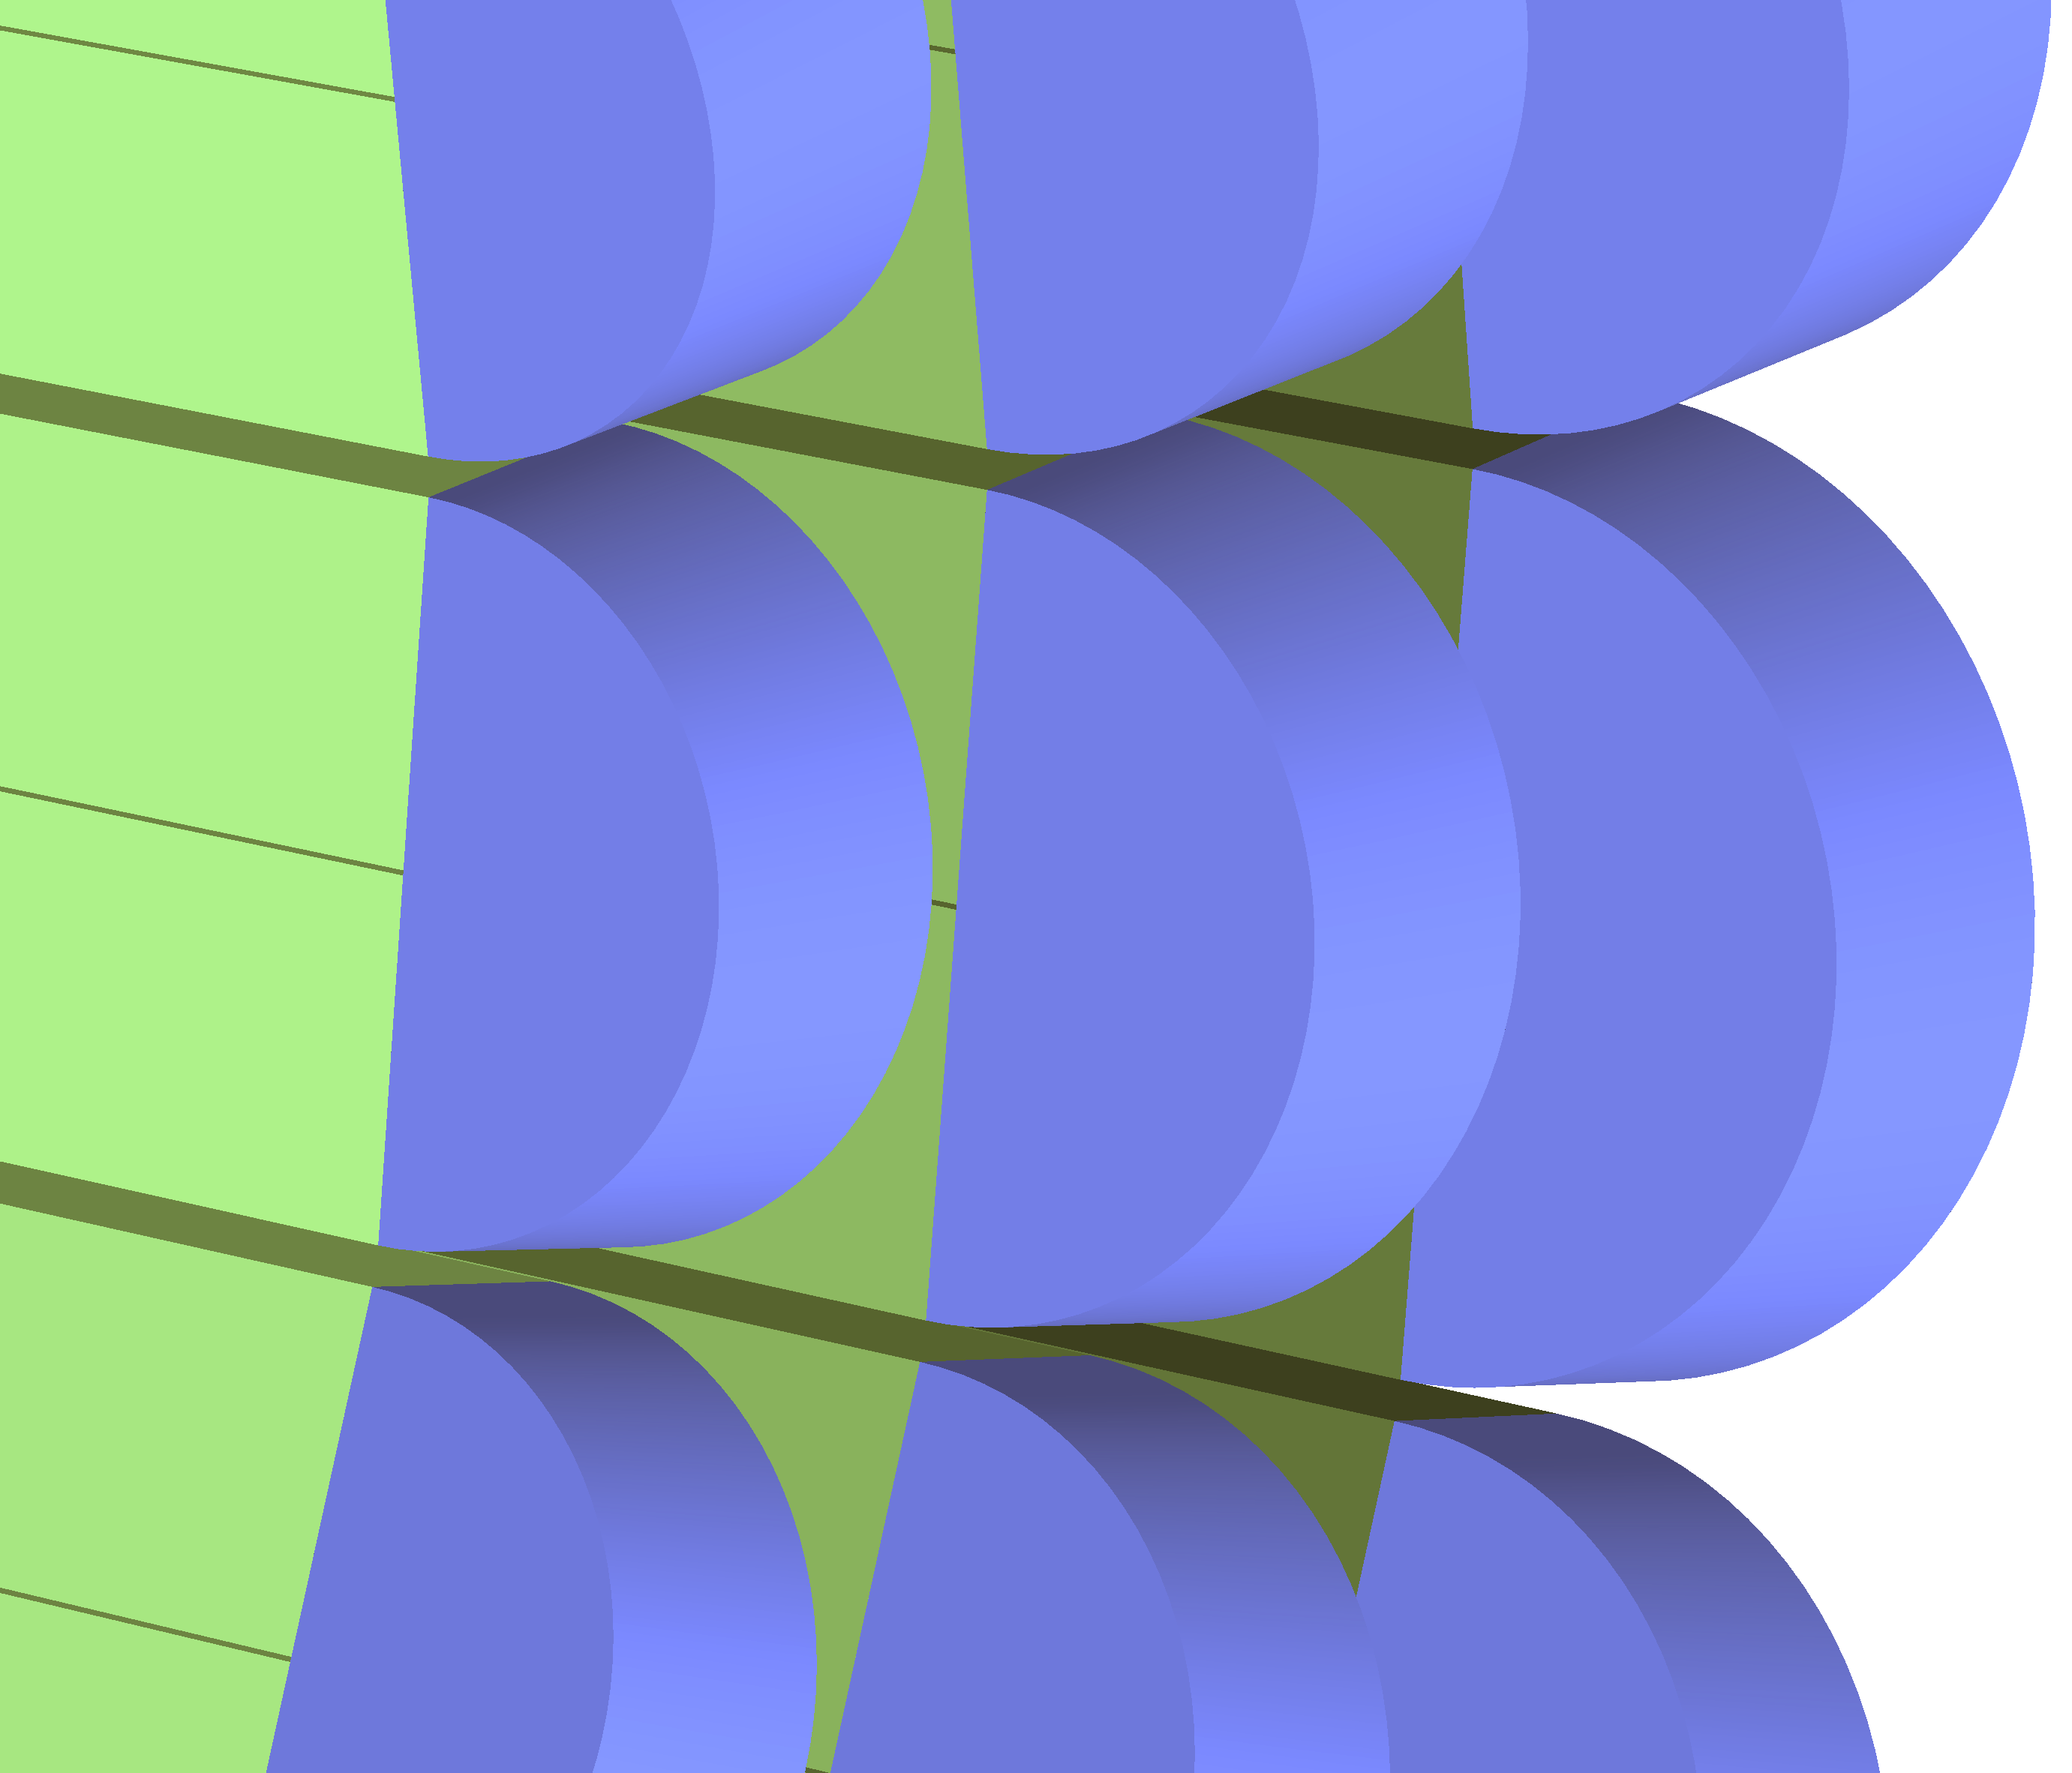
\includegraphics[width=0.95\columnwidth,keepaspectratio]{img/cndDetail.png}
	\caption{Top: overall view of the CND detector. Three layers of scintillators are placed at increasing z. Pairs of scintillators
            are connected through a scintillator u-shaped junction. Bottom: enlarged view of the junctions. }
	\label{fig:cndGeometry}
\end{figure}


\subsubsection{Geometry Git Location}
The github location of the gemc perl api script is \url{https://github.com/gemc/detectors/tree/master/clas12/cnd}.


\subsection{Digitization}

\subsubsection{ADC}

The energy deposited is reduced based on the position on the paddle using the calibration attenuation length. Two signals are then propagated, one directly
to the PMT and one through the scintillator junction. A $30\%$ factor takes into account losses at junctions.

The corrected energy is converted to the theoretical number of photos $N_{th}$ using the constant $1210 \gamma / MeV $. A poissonian is used to
calculate the actual number of photons $N_{actual}$ and the resulting ``smeared`` energy is the converted to adc using the FADC conversion factor.

\subsubsection{TDC}

The absolute hit time is corrected by:

\begin{itemize}
	\item the effective velocity (from CCDB)
	\item a left/rigth time offset factor (from CCDB)
	\item the Birks Attenuation factor
\end{itemize}

The time is then smeared by a $\sigma$ resolution read from CCDB using a gaussian function and then digitized using a TDC conversion factor.


\subsubsection{Summary of CCDB Table used}
\begin{itemize}
	\item /calibration/cnd/Status\_LR
	\item /calibration/cnd/TDC\_conv
	\item /calibration/cnd/Attenuation
	\item /calibration/cnd/EffV
	\item /calibration/cnd/Energy
	\item /calibration/cnd/UturnTloss
	\item /calibration/cnd/TimeOffsets\_LR
	\item /calibration/cnd/TimeOffsets\_layer
\end{itemize}



\subsection{Digitized Bank}
The digitized output bank has $ID=300$, and the variables are summarized in Table \ref{tab:cndBank}

\begin{table}[h]
	\begin{center}
		\begin{tabular}{| c | c | c |}
			\hline \hline
			Variable         & Description  & Tag  \\
			\hline
              sector  &                                     sector number  &    1   \\
               layer  &                                      layer number  &    2   \\
           component  &                                  component number  &    3   \\
                ADCL  &                                          ADC Left  &    4   \\
                ADCR  &                                         ADC Right  &    5   \\
                TDCL  &                                          TDC Left  &    6   \\
                TDCR  &                                         TDC Right  &    7   \\
                hitn  &                                        hit number  &   99   \\
			\hline \hline
		\end{tabular}
	\end{center}
	\caption{The digitized CND bank}\label{tab:cndBank}
\end{table}


\subsubsection{Time Window}
The timewindow of the CND is set to 5 ns.


\subsubsection{Process Routine Git Repository Location}
The CND hit process routine location in git is \url{https://github.com/gemc/source/blob/master/hitprocess/clas12/cnd_hitprocess.cc}
